%; whizzy chapter -dvi
% -initex iniptex -latex platex -format platex -bibtex jbibtex -fmt fmt
% 以上 whizzytex を使用する場合の設定。
 
%     Tokyo Debian Meeting resources
%     Copyright (C) 2012 Junichi Uekawa
%     Copyright (C) 2011 Nobuhiro Iwamatsu

%     This program is free software; you can redistribute it and/or modify
%     it under the terms of the GNU General Public License as published by
%     the Free Software Foundation; either version 2 of the License, or
%     (at your option) any later version.

%     This program is distributed in the hope that it will be useful,
%     but WITHOUT ANY WARRANTY; without even the implied warranty of
%     MERCHANTABILITY or FITNESS FOR A PARTICULAR PURPOSE.  See the
%     GNU General Public License for more details.

%     You should have received a copy of the GNU General Public License
%     along with this program; if not, write to the Free Software
%     Foundation, Inc., 51 Franklin St, Fifth Floor, Boston, MA  02110-1301 USA

%  preview (shell-command (concat "evince " (replace-regexp-in-string "tex$" "pdf"(buffer-file-name)) "&"))

%%ここからヘッダ開始。

\documentclass[mingoth,a4paper]{jsarticle}
\usepackage{monthlyreport}
% 日付を定義する、毎月変わります。
\newcommand{\debmtgyear}{2014}
\newcommand{\debmtgmonth}{08}
\newcommand{\debmtgdate}{23}
% started from zero:
% (let ((year 2013) (month 7)) (+ (* (- year 2005) 12) month -1))
\newcommand{\debmtgnumber}{116}

\begin{document}

\begin{titlepage}
\thispagestyle{empty}
% タイトルページ:編集必要な部分は最初のマクロに飛ばすこと

\vspace*{-2cm}
第\debmtgnumber{}回 東京エリア Debian 勉強会資料\\
\hspace*{-2cm}

\includegraphics{image2012-natsu/dotdeb.pdf}\\
\hfill{}\debmtgyear{}年\debmtgmonth{}月\debmtgdate{}日

% ここはアップデートすること
% 全角文字にしないとフォントのサイズが合わないので注意
\rotatebox{10}{\fontsize{30}{30} {\gt 特集:Debianでタイルマップサービス}}\\

\vspace*{-2cm}
\hfill{}
\includegraphics[height=6cm]{image200502/openlogo-nd.eps}
\end{titlepage}

\newpage

\begin{minipage}[b]{0.2\hsize}
 \definecolor{titleback}{gray}{0.9}
 \colorbox{titleback}{\rotatebox{90}{\fontsize{80}{80} {\gt デビアン勉強会} }}
\end{minipage}
\begin{minipage}[b]{0.8\hsize}
\hrule
\vspace{2mm}
\hrule
\begin{multicols}{2}
\tableofcontents
\end{multicols}
\vspace{2mm}
\hrule
\end{minipage}

\dancersection{事前課題}{野島 貴英}

今回の事前課題は以下です:
\begin{enumerate}
 \item 本日、何の作業をやるかを宣言ください。
\end{enumerate}
この課題に対して提出いただいた内容は以下です。
\begin{multicols}{2}
{\small
\begin{prework}{ dictoss(杉本 典充) }
\begin{itemize}
\item 前回のパッケージング道場の続きをする
\item VAIO Pでlinux-image-3.14の場合にMP3再生が倍速再生されるバグの調査
\end{itemize}
\end{prework}

\begin{prework}{ 吉野(yy\_{}y\_{}ja\_{}jp) }
DDTSS
\end{prework}

\begin{prework}{ zinrai }
iodine,nikolaを使ってみる。\\
\url{https://packages.debian.org/sid/iodine}\\
\url{https://packages.debian.org/sid/nikola}
\end{prework}

\begin{prework}{ 田上 健太 }
新しく個人用ノートPCを買ったので、開発環境を構築していきます。
\end{prework}

\begin{prework}{ 野島 貴英 }
xmrisパッケージ化やる。
\end{prework}

\begin{prework}{ wbcchsyn }
6月に発表したツールについて、頂いた意見の取り込みとフィードバックをおこないます。
\end{prework}

\begin{prework}{ まえだこうへい }
\url{http://d.palmtb.net/pages/about.html#todo-from-maintainer-dashboard}
のバグ潰し
\end{prework}

\begin{prework}{ 野首(@knok) }
\begin{itemize}
\item KAKASIのローマ字テーブル見直し
\item Leap Motion, HID送信機のハック
\item ECS Livaの問題調査
\end{itemize}
\end{prework}

}
\end{multicols}

\dancersection{Debian Trivia Quiz}{野島 貴英}

ところで、みなさん Debian 関連の話題においついていますか?Debian関連の話
題はメーリングリストをよんでいると追跡できます。ただよんでいるだけではは
りあいがないので、理解度のテストをします。特に一人だけでは意味がわからな
いところもあるかも知れません。みんなで一緒に読んでみましょう。

今回の出題範囲は\url{debian-devel-announce@lists.debian.org} や \url{debian-devel@lists.debian.org}に投稿された
内容などからです。

\begin{multicols}{2}
%; whizzy-master ../debianmeetingresume201311.tex
% 以上の設定をしているため、このファイルで M-x whizzytex すると、whizzytexが利用できます。
%

\santaku
{2014/8/16にDebianは誕生日を迎えました。さて今年で何歳?}
{25}
{21}
{20}
{B}
{1993/8/16にIan Ashley Murdockさんにより、Debianは創設されました。というわけで、21歳です。Debian Dayはもう過ぎちゃいましたが、本日(2014/8/23)の勉強会後の宴会で祝いたいと思います!}

\santaku
{2014/7時点の各国のアクティブなDebian Developerの数とそれぞれの国の人口との比率が最も多いのはどこの国?}
{Finland}
{Ireland}
{New Zealand}
{A}
{Finlandは本割合は2009年からずっと毎年1位(今年3.61ppm。)2位 Ireland 3位 New Zealand。日本の本割合は0.28ppmで30位でした。単にアクティブDeveloperの絶対数が多い国は1位USA、2位Germany、3位France。}

\santaku
{OpenAmbitが2014/7にパッケージ化されsidへリリースされました。ところで何するパッケージ?}
{AmazonTV用アプリ開発環境}
{ChoromeCast用アプリ開発環境}
{SUNNTO AMBIT用アプリ開発環境}
{C}
{SUNNTO AMBITという腕時計型のGPS搭載の端末のアプリ開発環境となります。楽天とか、Amazonで買えます。スポーツ好きな方はDebianでアプリ開発やってみてください。}

\santaku
{2014/7/31にtechnical committeeによりDebianのデフォルトのJPEG圧縮伸長ライブラリとして採択されたのは以下のうちのどれ?}
{libjpeg6b}
{libjpeg8/9}
{libjpeg-turbo}
{C}
{libjpeg-turboはlibjpeg6 ABI互換のJPEG圧縮伸長ライブラリで、libjpeg6を遥かに凌ぐ速さで動作します。ここで、JPEG圧縮伸長ライブラリのデフォルトとして、libjpeg8/9か、libjpeg-turboかで議論が分かれていましたが、technical comitteeはlibjpeg-turboをデフォルトのJPEG圧縮伸長ライブラリとしました。}

\santaku
{2014/7/31にtechnical committeeから、「Debianパッケージは複数のinitシステムに対応する事」ということが再アナウンスされました。何のパッケージのドタバタがきっかけでしょう?}
{ftp}
{tftp-hpa}
{ncftp}
{B}
{experimentalにtftp-hpa 5.2-17が入ったが、そのchangelogとして''Removing upstart hacks, they are ugly and upstart is dead now.''という内容が入っていた件が物議を醸しました。bug746715参照。}

\santaku
{2014/7/20にsqueeze(注:squeeze-ltsではない)の最後のアップデートが行われました。何回目のアプデートでしょうか?}
{10}
{9}
{8}
{A}
{最後のsqueezeのアップデートです。実はこのアップデートを行っても、Debianですでに報告されているsqueezeのセキュリティホールの一部は残ったままです。しかしながら、これ以上のアップデートは無いので、wheezyにアップデートするか、squeeze-ltsの採用を検討しましょう。}

\santaku
{2014/7/31にJessieに搭載の可能性のあるlinux kernelのバージョンのアナウンスが行われました。バージョンはいくつでしょう?}
{3.14}
{3.12}
{3.16}
{C}
{2014/8/14にkernel.orgでlinux kernel3.16のリリースがアナウンスされました。Debian Kernelチームのアナウンスでは、「3.16がJessieに採用される可能性があるので、現在のパッケージが3.16と互換のあるKernel APIの元で動作するか確認し、問題があれば然るべき対応してほしい」とのこと。}

\santaku
{VCS-*フィールドのVCS情報を参照し、パッケージのchangelogが合致しているかのチェックが行われるようになりました。以下のどのサイトで確認できる?}
{http://qa.debian.org/cgi-bin/vcswatch}
{http://bugs.debian.org/}
{http://codesearch.debian.net/}
{A}
{vcswatchのページにアクセスし、見たいパッケージ名入れると、状況が得られます。詳しくはvcswatchのサイトの説明をご覧ください。}

\santaku
{パッケージに含まれているドキュメントに関して、lintianが新たな警告をするようになりました。以下のどれ?}
{HTMLファイル中の画像/CSS/JS/videoリンクがローカルファイルを指していない場合、警告}
{HTMLファイル中のDebianの綴りが間違っている場合、警告}
{HTMLファイルが入っていない場合、警告}
{A}
{ブラウザがHTMLファイルを表示する場合、ローカルのファイルであっても、表示時にブラウザが自動でリンク先をアクセスしてしまう作用を持つリンクがあります。ここに外部サイトのURLが入っていた場合、その外部サイトは、HTMLファイルが閲覧された時の情報を収集することが出来てしまいます。こういったことはセキュリティ上良くないので、該当するようなHTMLファイルが含まれている場合、lintianが警告するようになりました。}

\santaku
{2014/7にBTSのWEBサイトにreplyのリンクがつくようになりました。このリンクをブラウザからクリックすると何が起きるようになった?}
{BTS上でreplyしている次のメッセージが表示されるようになった。}
{BTS上のreply用のフォームがブラウザに表示されるようになった。}
{メーラが起動し、正しいSubject/宛先/引用が入るようになった。}
{C}
{やってみれば判りますが、Bugレポートに対する返答をする場合に、非常に便利です。BTSから見て、正しい内容と宛先で、返答出来るように下書きメールがメーラに準備されるようになりました。}

\santaku
{2014/8/14にDebian Installer Jessie Beta 1がアナウンスされました。このバージョンのインストーラで導入されるinitシステムは結局どうなった?}
{systemdになった}
{sysvinitになった}
{upstartになった}
{A}
{このバージョンのDebian Installerから、initシステムとしてsystemdが入るようになりました。ちなみにこの件、Installerプログラム本体の話であって、Jessie本体のBeta版リリースという意味では無い事に注意。}

\end{multicols}

\dancersection{最近のDebian関連のミーティング報告}{野島 貴英}

\subsection{第115回東京エリアDebian勉強会with第2回Debianパッケージング道場報告}

\begin{itemize}
\item  (株)サイバーエージェントさんをお借りしての開催でした。途中参加の方も含め参加者10名。
\item 10:00-16:00までは第2回Debianパッケージング道場を岩松さんにより進行、
\item 16:00以降はいつもの東京エリアDebian勉強会の形式で、前田さんにより「Jenkinsを
用いたパッケージ作成の自動化」の発表
\end{itemize} 

 でした。

 パッケージ作成については公式Debian Developerの方による最近の事情も含めた説明が行われ、また、
Jenkinsを使いパッケージの生成を最後まで自動化されているのは素晴らしかったです。

 最後に会場近くの飲み屋で宴会をしました。

% % (query-replace-regexp "<.*?>" "")
% % (query-replace-regexp "^[	 ]\+" "")

%-------------------------------------------------------------------------------
\dancersection{Debianでタイルマップサービス作ってみた}{なかおけいすけ}
%-------------------------------------------------------------------------------
\index{debian-tilemap-service}

%NASA主催のInternational Space App Challengeという宇宙をネタにした
%アプリをつくるハッカソンで、地球観測衛星のデータを可視化してOpenStreetMapに
%オーバーレイできるタイルマップサービスを、Debianで開発しましたので紹介します。

\subsection{タイルマップサービスとは}
タイルマップサービス (TMS: Tile Map Service)は、OSGeo財団(Open Source Geospatial Foundation)が策定した、地図をタイルとして提供するプロトコルです。
タイルは、地図を領域とズームレベル毎に256px $\times$ 256pxの画像に分割した
もので、図\ref{fig:tile_pylamid}のようにピラミッド構造になっています。
大きな画像を小分割することで、必要な領域、ズームレベルだけを取得し、不要になった部分を
開放することで、メモリの消費量を削減し、効率良く通信を行うことができます。
タイルは、ズームレベルが一つ大きくなると、表示する範囲が$1/4$になります。
例えば、ズームレベル0では、地球全体を1枚のタイルで表し、ズームレベル1では4枚、
ズームレベル2では16枚....ズームレベルnでは$2^n \times 2^n$枚になります。
ズームレベル16になると、$2^{32} = 4,294,967,296 \simeq 4.3 \times 10^9$枚もの
タイルが必要になります。
%
\begin{figure}[hbp]
\centering
\includegraphics{image201408/Tiling.eps}
\caption{タイルのピラミッド構造\cite{ref:tile}}
\label{fig:tile_pylamid}
\end{figure}

タイルは、HTTPで、\texttt{http://BASEURL/VERSION/TILENAME/z/x/y.png} という形式のURIで取得できます。現在、VERSIONは1.0.0です。
ここでzはズームレベル、x、yは領域を表す整数です。x、yは、$lat$、$lon$を緯度、経度として
以下のように書けます\cite{ref:tilename}。
\begin{eqnarray*}
x &=& \frac{2^z(lon + 180)}{360}\\
y &=& 2^{z-1}(1-\frac{\ln(\tan(lat\frac{\pi}{180})) + \frac{1}{\cos(lat\frac{\pi}{180})}
}{\pi})
\end{eqnarray*}

\subsection{タイルの生成}
タイルを生成するためには、表示するデータが必要です。今回はJAXAの
水循環変動観測衛星「しずく」に搭載されているAMSR2というセンサーで観測された
海水表面温度データをタイルにしてみましょう。

「しずく」のデータは、登録が必要ですが一般公開されています\cite{ref:gcom_w1}。
登録をすると、sftpでデータをダウンロードできます。
%
\begin{commandline}
$ sftp -oPort=2051 username@gcom-w1.jaxa.jp
sftp> get AMSR2/YYYY/YYYY.MM/L3/SST_10/1/GW1AM2_YYYYMMDD_01D_EQOD_L3SGSSTHA1100100.h5.gz
\end{commandline}
%
ダウンロードしたファイルは、gzipで圧縮されたHDF5というファイルフォーマットの
数値データです。HDF5は科学技術用に開発された数値データを格納するためのバイナリーフォーマットで
多次元の数値データだけでなく、観測日時や観測者、スケーリングファクタ、解析アルゴリズムといった
情報を階層構造で格納することができるフォーマットです。もちろん仕様は公開されており
PythonやRubyのモジュールもあります。

この中に海水面温度の数値データが北緯0度、東経0度から0.1度刻みのメッシュで格納されています。
まずこのメッシュ1つを1pxとする画像を作ります。そうすると地球全体で3600px$\times$1800px
の画像ができます。

私はPythonを使って、メッシュのデータを取り出し、あらかじめ作っておいたカラーマップで
数値をRGBに変換し、ASCIIテキストでピクセルを表現できるPPMで出力しました。
欠損値は(R,G,B)=(0,0,0)としています。
\begin{figure}[hbp]
\centering

\includegraphics{image201408/map.eps}
\caption{生成したマップ}
\label{fig:map}
\end{figure}

この画像をImageMagickのconvertコマンドでtiff画像にしつつ、欠損値を表す黒を
透明に変換します。
\begin{commandline}
$ convert -transparent black converted.ppm map.tiff
\end{commandline}

ここでできるTiff画像(図\ref{fig:map})は、地図ではありますが、ピクセルと緯度経度の対応関係の情報を持っていません。
そこでGDALを使って、このTiff画像を位置情報を持つGeoTiffというフォーマットに変換します。
GDALは、地理空間データのスイスアーミーナイフ的な存在で、
GeoTiffやJPG、PNGといったラスタデータフォーマットやHDF、NetCDF等のファイルを読んで
他のフォーマットに変換したり、測地系の変換等を行うことができるライブラリ、ユーティリティ群です。
(ここまででやってきた、HDF5ファイルから数値データを取り出してカラーマップにする
ことも、GDALだけでできる気がします。)
GDALは、gdal-binというパッケージになっています。TiffファイルをGeoTiffに変換するには、
gdal\_translate コマンドで、緯度経度が分かっているピクセルを教えてあげます。
そしてgdalwarpコマンドで、gdal\_translateで指定したピクセルと緯度経度を元に
幾何変換して測地系の情報を追加します。
%
\begin{commandline}
$ gdal_translate -q -gcp 0 0 0 90 \
                -gcp 3600 0 360 90 \
                -gcp 0 1800 0 -90 \
                -gcp 3600 1800 360 -90 map.tiff tmp.tiff

$ gdalwarp -q -s_srs EPSG:4326 -r cubic tmp.tiff map.tiff
\end{commandline}
%
各ピクセルが位置情報を持った画像ファイルが完成しました!
これでようやくタイルを生成する準備ができました。

タイルの生成には、python-gdalパッケージの gdal2tiles.py コマンドを使います。
ただこのコマンドは、指定したズームレベルのタイルをすべて生成してしまいます。
前述の通り、ズームレベルを増やすと指数関数的に生成する画像が増えていくので
タイルの生成に数時間かかってしまいます。
数時間かけて苦労してタイルを作っても、現実にはユーザーがすべてのタイルを
見てくれるわけではありません。だったら必要なタイルだけを、必要な時に生成すれば
良いのです。

\subsection{タイルマップサーバの実装}
では、リクエストがあったときに必要に応じてタイルを生成するサーバーを作りましょう。
今回はWebサーバはApacheで、mod\_pythonとmod\_rewriteを用います。
mod\_rewriteの説明は不要でしょう。正規表現にマッチしたリクエストのURLを
書き換えるモジュールです。

mod\_python は、ApacheのPython bindingで、CGIの置き換えを目的としたモジュールです。
インストールするには、以下のコマンドを実行します。
\begin{commandline}
# apt-get install libapache2-mod-python
# a2enmod python
# service apache2 restart
\end{commandline}
設定は、/etc/conf.d/ の中に適当なファイル名のファイルを作って
\begin{commandline}
<Directory /some/path>
  SetHandler mod_python
  PythonHandler mod_python.publisher
</Directory>
\end{commandline}
としすればよいでしょう。

mod\_pythonのmod\_python.publisherは、HTTPリクエストをPythonの
関数の呼び出しに変換します。
たとえば、www.example.org のDocumentRootに、hello.pyという
以下のPythonスクリプトがあったとしましょう。
\begin{commandline}
def sayHello(req, name):
  return ``Hello %s''%name
\end{commandline}
もしも、\url{http://www.example.org/hello.py/sayHello?name=Debian}にGET
リクエストがあると、Webサーバは、sayHello関数のname引数にDebianを代入して
sayHello関数を呼び出し、''Hello Debian''と表示されます。

タイルマップサービスにアクセスするクライアントは、
\url{http://BASEURL/VERSION/TILENAME/z/x/y.png}というURIでGETしようと
するので、mod\_rewriteでURIを書き換えましょう。たとえば、\url{www.example/org}の
/etc/apache/conf.dに以下のように設定すると、
%
\begin{commandline}
<Directory "/var/www/tile/1.0.0/sst">
	RewriteEngine	On
	RewriteBase	/tile/1.0.0/sst/
	RewriteRule	^([0-9]+)/([0-9]+)/([0-9]+).png    gettile.py/get?z=$1&x=$2&y=$3

	AddHandler	mod_python    .py
	PythonHandler	mod_python.publisher
</Directory>
\end{commandline}
%
\url{http://www.example.org/tile/1.0.0/sst/4/12/34.png}が、
\url{http://www.example.org/tile/1.0.0/sst/gettile.py/get?z=4&x=12&y=34}
に変換されるので、gettile.pyの中の、req, x, z, yの引数をとる関数が呼び出されます。
ここに指定されたURIのタイルだけを生成処理を書けば、オンデマンドにタイルを生成する
タイルマップサービスができます。


単一タイルだけを生成するには、gdal2tiles.pyを少し修正します。
generate\_base\_tiles関数の中の
1180行目付近にすべてのタイルを作っているループが存在するので、

\begin{commandline}
     def generate_base_tiles(self):
         """Generation of the base tiles (the lowest in the pyramid) directl y from the input raster"""

                               (Snip...)

         for ty in range(tmaxy, tminy-1, -1): #range(tminy, tmaxy+1):
             for tx in range(tminx, tmaxx+1):
 
                 if self.stopped:
                     break
                 ti += 1
                 tilefilename = os.path.join(self.output, str(tz), str(tx), "%s.%s" % (ty, self.tileext))
                 if self.options.verbose:
                     print(ti,'/',tcount, tilefilename) #, "( TileMapService     : z / x / y )"
\end{commandline}

それをひも解いて指定されたタイルを生成している部分を、関数として抜き出します。
\begin{commandline}
     def generate_base_tiles(self):
         """Generation of the base tiles (the lowest in the pyramid) directl y from the input raster"""

                               (Snip...)

         for ty in range(tmaxy, tminy-1, -1): #range(tminy, tmaxy+1):
             for tx in range(tminx, tmaxx+1):
                 generate_tile(tx, ty, self.tmaxz)
 
     # -------------------------------------------------------------------------
     def generate_tile(self, ty, tx, tz):
         ds = self.out_ds
         tilebands = self.dataBandsCount + 1
         querysize = self.querysize
\end{commandline}

あとは、generate\_tile関数を、mod\_pythonが呼ぶスクリプトから呼べば
できあがりです。
\begin{commandline}
def get(req, z, tx, ty):
        req.content_type = 'image/png'
        #req.write('z: %s\ntx: %s\nty: %s'%(z,tx,ty))

        g = GDAL2Tiles(['/home/chome/public_html/tile/sst/map.tiff','/var/www/tile/1.0.0/sst'])
        g.open_input()
        g.generate_tile(int(ty),int(tx),int(z))

        with open('/var/www/tile/1.0.0/sst/%s/%s/%s.png'%(z,tx,ty), 'rb') as f:
                req.write(f.read())
\end{commandline}

\subsection{まとめ}
Debianでパッケージングされているオープンソースのプログラムやライブラリを組み合わせて
タイルマップサービスを作ってみました。
gdal2tiles.pyを少し修正しmod\_pythonから呼ぶことによって、オンデマンドで
必要なタイルだけを生成しています。

今回開発したサービスは\url{http://www.hi-rezclimate.org}で公開されています。
データの取得、GeoTiffにするところまでは自動化されているので、毎日最新のデータをダウンロードして自動で更新されています。「しずく」は海水面温度だけでなく、海上風速や水蒸気量、積雪深といった水に関する現象を観測しています。今後サポートするデータを増やしていく予定です。



\begin{thebibliography}{9}
\bibitem{ref:tile}``Tile Map Service in Geoide'', \url{http://geoikia.idgis.eu/wiki-english/index.php/Tile\_Map\_Services\_in\_Geoide}
\bibitem{ref:tilename} ``Slippy map tilenames'', \url{http://wiki.openstreetmap.org/wiki/Slippy\_map\_tilenames}
\bibitem{ref:gcom_w1} GCOM-W1 データ提供サービス \url{https://gcom-w1.jaxa.jp/auth.html}
\end{thebibliography}
\printindex

\cleartooddpage

\vspace*{15cm}
\hrule
\vspace{2mm}

\includegraphics[width=2cm]{image200502/openlogo-nd.eps}
\noindent \Large \bf Debian 勉強会資料\\
\noindent \normalfont \debmtgyear{}年\debmtgmonth{}月\debmtgdate{}日 \hspace{5mm}  初版第1刷発行\\
\noindent \normalfont 東京エリア Debian 勉強会 (編集・印刷・発行)\\
\hrule

\end{document}
